\subsubsection{Modificar Refacción}
En la figura \ref{fig:Diagrama de Secuencia - Modificar Empleado} se muestra el flujo de las diversas actividades que corresponden a la modificación de los datos de una refacción que se encuentra en almacén del taller, esto en dado caso que haya un error en la captura de dichos datos. En este proceso, el administrador solicita esta modificación a través del sistema y este mismo interactúa con la base de datos para su modificación. En este proceso existen tres variantes para los datos a modificar:
\begin{itemize}
	\item \textbf{Existe empleado:} Se asegura que la refacción está registrada,en dado caso que si, se procede a la modificación del mismo mediante un formulario de actualización.
	\item \textbf{No existe el empleado:} Si no existe el registro de la refacción en la base de datos, el sistema muestra un mensaje de error al usuario.
	\item \textbf{Datos válidos:} Al modificar los datos de un empleado, el sistema valida si esa información es correcta, es decir, si los campos han sido llenados y el formato es el correspondiente con cada uno de dichos campos.
	\item \textbf{Datos no válidos:} Los datos que se quieren sobrescribir en la base de datos son incorrectos y el sistema no permite la actualización y muestra un mensaje de error.
\end{itemize}
\begin{figure}[!h]
	\centering
	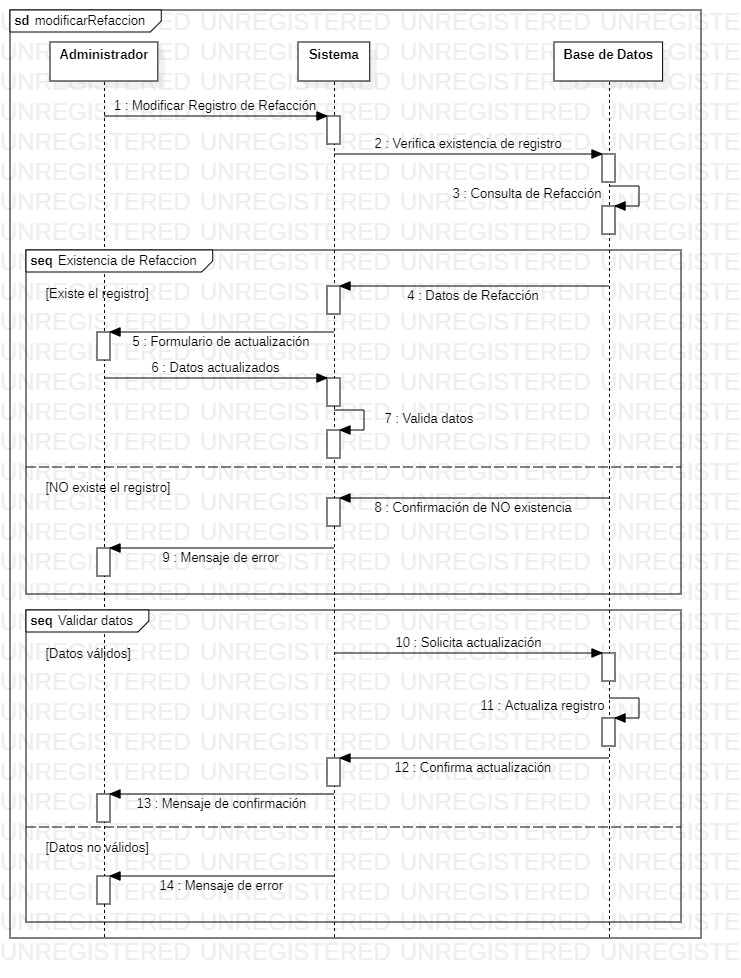
\includegraphics[width=1\textwidth]{./diseno/vprocesos/imagenes/modificarRefaccion}
	\caption{Diagrama de Secuencia - Modificar Refacción}
	\label{fig:Diagrama de Secuencia - Modificar Refaccion}
\end{figure}
\clearpage